\chapter{Pruebas de rendimiento}\label{cap:rendimiento}
\noindent En este cap\'itulo analizaremos el rendimiento de la propuesta sobre un des\-plie\-gue real, describiendo brevemente el entorno de ejecuci\'on y, posteriormente, exponiendo y ana\-li\-zan\-do los resultados obtenidos.

\section{Entorno de prueba}\label{sec:entornodeprueba}
\noindent La figura \ref{fig:clusterdespliegue} muestra la configuraci\'on concreta del cl\'uster de ejecuci\'on. La parte izquierda de la imagen contiene el nodo \emph{controlador} del cloud; la parte derecha el nodo \emph{Nodo de cloud}. En el nodo controlador se ha realizado una instalaci\'on completa de OpenStack Folsom ---pero sin \texttt{Cinder}, \texttt{Swift} o \texttt{Quantum}---, \texttt{MySQL} ---para soportar la persistencia de los objetos tanto de OpenStack como de \texttt{Django}---, \texttt{Fabric} y \texttt{Qpid} como cola de mensajes para OpenStack. En el Nodo de Cloud se ha instalado lo m\'inimo requerido para ejecutar instancias virtuales: el m\'odulo \texttt{Compute}. Para cubrir el resto de la funcionalidad como el recuento de recursos disponibles, la seguridad de acceso o los detalles de las instancias o de las im\'agenes, el Nodo de Cloud se apoya en el controlador utilizando Qpid como medio de comunicaci\'on as\'incrona.\newline

\begin{figure}[tbp]
\begin{center}
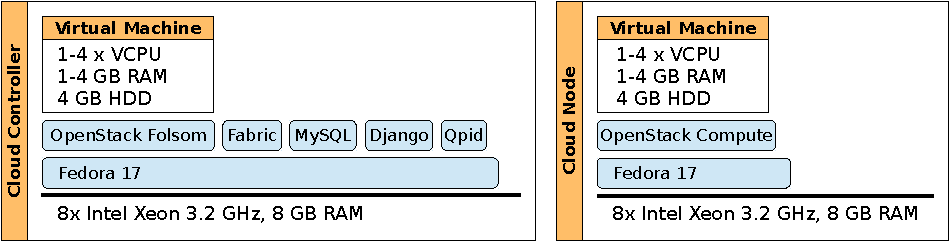
\includegraphics[width=0.99\textwidth]{imagenes/038.pdf}
 \caption{Morfolog\'ia del despliegue}
\label{fig:clusterdespliegue}
\end{center}
\end{figure}

En cuanto al hardware, ambos nodos poseen la misma configuraci\'on f\'isica que, sin entrar en detalle, alberga un \emph{Xeon} de ocho n\'ucleos a 3.20 \emph{GHz} con VT-x, 8 GB de RAM, un disco duro de 200 GB SATA 3 Gb/s 7200 RPM y conectividad de red a 1 Gb/s.

La elaboraci\'on de la imagen que se carga en la m\'aquina virtual y que soporta la ejecuci\'on, se hab\'ia detallado en la secci\'on \ref{subsec:maquinavirtual}. La versi\'on de \texttt{Hadoop} utilizada es la 1.0.4 y la de \texttt{JRE} la 1.7v6. \newline

La figura \ref{fig:clusterdespliegue} tambi\'en muestra la m\'aquina virtual soporte de ejecuci\'on para Hadoop. A esta m\'aquina virtual o instancia en ejecuci\'on se le conceder\'an entre 1 y 4 GB de RAM e id\'entico n\'umero de CPUs virtuales, conformando distinos casos de prueba que evaluar\'an la escalabilidad de la soluci\'on. La cantidad de RAM asignada en cada caso ser\'a compartida por el SO hu\'esped y la m\'aquina virtual Java sobre la que se ejecuta Hadoop. El des\-plie\-gue del cl\'uster virtual Hadoop se ha configurado de forma que la m\'aquina virtual Java tenga acceso a toda la RAM de las instancias; ser\'ia te\'oricamente posible que alguna ejecuci\'on de Hadoop se quedase corta de memoria RAM virtual, sobre todo en los casos con 1 GB solamente, forzando la transferencia de p\'aginas de memoria RAM virtual a disco duro virtual, lo que se traducir\'ia en una reducci\'on del ancho de banda de trabajos.

\section{Metodolog\'ia de prueba}\label{sec:metodologiaprueba}
\noindent Se pretende medir la \emph{escalabilidad} de la soluci\'on, tanto \emph{horizontal} como \emph{vertical}, y estudiar su comportamiento ante trabajos MapReduce de dificultad creciente. Para analizar su escalabilidad, fijaremos un problema a la entrada lo suficientemente grande como para que todas las instancias reciban peticiones de procesamiento. El problema en cuesti\'on consiste en contar el n\'umero de palabras ---usando el ya comentado \texttt{wordcount}--- en 62.5 MB de texto plano. \newline 

Concretamente, para analizar la escalabilidad horizontal ---entendida como la variaci\'on del tiempo de ejecuci\'on de un problema en un cl\'uster al ir incrementando el n\'umero de nodos (idealmente id\'enticos)--- crearemos desde una hasta ocho m\'aquinas virtuales de 1 GB de RAM, doblando el n\'umero de m\'aquinas virtuales hasta las ocho. Para analizar la escalabilidad vertical ---entendida como la variaci\'on del tiempo de ejecuci\'on de un problema en un cl\'uster al ir incrementando las capacidades operativas de los nodos--- crearemos dos m\'aquinas virtuales de 1 GB de RAM cada una, e iremos doblando la RAM de las m\'aquinas virtuales hasta 4 GB. Finalmente, para estudiar la evoluci\'on de la soluci\'on ante problemas de distinto tama\~no, se lanzar\'an ocho m\'aquinas virtuales de 1 GB de RAM y se duplicar\'a el volumen de datos a la entrada desde los 62.5 MB originales hasta los 250 MB.\newline

Todas las pruebas se har\'an \emph{en caliente}. \texttt{Glance} y \texttt{Compute} cooperan para \emph{cachear} el sistema de ficheros de las im\'agenes al ejecutarse, de forma que la latencia de creaci\'on es mayor la primera vez que se lanza una instancia de una imagen. Para evitar que se incluyan en las medidas esos valores \emph{en fr\'io} del cloud, se crear\'an y destruir\'an instancias de la imagen del proyecto antes de anotar los resultados. \newline

A priori, la variabilidad esperada de los resultados entre ejecuciones es lo suficientemente peque\~na como para fijar a \emph{diez} el n\'umero de realizaciones de cada caso de prueba ---esta suposici\'on a priori se ve confirmada a posteriori a la vista del resultado de los experimentos. Para ello se har\'an medidas auto\-ma\-ti\-za\-das, con marcas de tiempo directamente en el c\'odigo, que distinguir\'an los siguientes cinco tiempos de inter\'es:

\begin{description}
    \item[Despliegue:] tiempo transcurrido desde que se hace la petici\'on \emph{crear ins\-tan\-cia} hasta que se puede acceder a todas ellas.
  \item[Configuraci\'on:] tiempo necesario para que se establezca el marco de ejecuci\'on para Hadoop. Incluye el tiempo de transferencia y descompresi\'on de los datos de entrada a la m\'aquina virtual y a HDFS, y la configuraci\'on del cl\'uster virtual Hadoop conformado por todas las instancias creadas.
  \item[MapReduce:] tiempo dedicado por Hadoop a la ejecuci\'on del trabajo wordcount.
  \item[Borrado:] tiempo utilizado para limpiar el entorno de ejecuci\'on. No incluye el tiempo requerido por OpenStack para eliminar por completo las ins\-tan\-cias.
  \item[Total:] tiempo que transcurre desde que se inicia el despliegue hasta que finaliza la petici\'on de borrado de las instancias.
\end{description}

Notar que los resultados presentados hacen referencia a la media aritm\'etica de las diez ejecuciones para cada caso. 


\section{An\'alisis de resultados}\label{sec:analisisresultados}

\begin{figure}[tbp]
\begin{center}
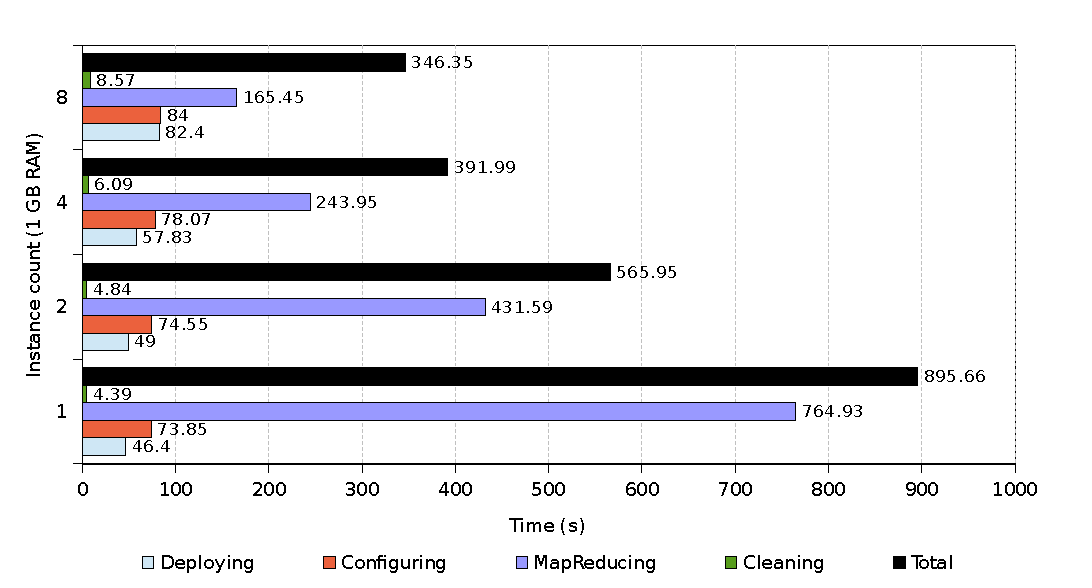
\includegraphics[width=0.98\textwidth]{imagenes/039.pdf}
\caption{Escalabilidad horizontal}
\label{fig:eschorizontal}
\end{center}
\end{figure}

\noindent La figura \ref{fig:eschorizontal} presenta la evoluci\'on de los distintos tiempos de inter\'es en funci\'on del n\'umero de instancias creadas, desde una hasta ocho. \newline

En ella se observa que los tiempos de despliegue, configuraci\'on y borrado aumentan ligeramente con el n\'umero de instancias desplegadas, mientras el tiempo de procesamiento se ve reducido. Esto es, el despliegue, la con\-fi\-gu\-ra\-ci\'on y el borrado dependen solamente del tama\~no del cl\'uster virtual; por el contrario, el tiempo MapReduce ---y por lo tanto tambi\'en el tiempo total--- depende adem\'as del volumen del trabajo a ejecutar. La figura \ref{fig:escvertical} presenta la evoluci\'on de los cinco tiempos de inter\'es a medida que se aumentan la cantidad de RAM y las CPUs virtuales de las dos instancias creadas; desde 1 GB y 1 VCPU hasta 4. \newline

\begin{figure}[tbp]
\begin{center}
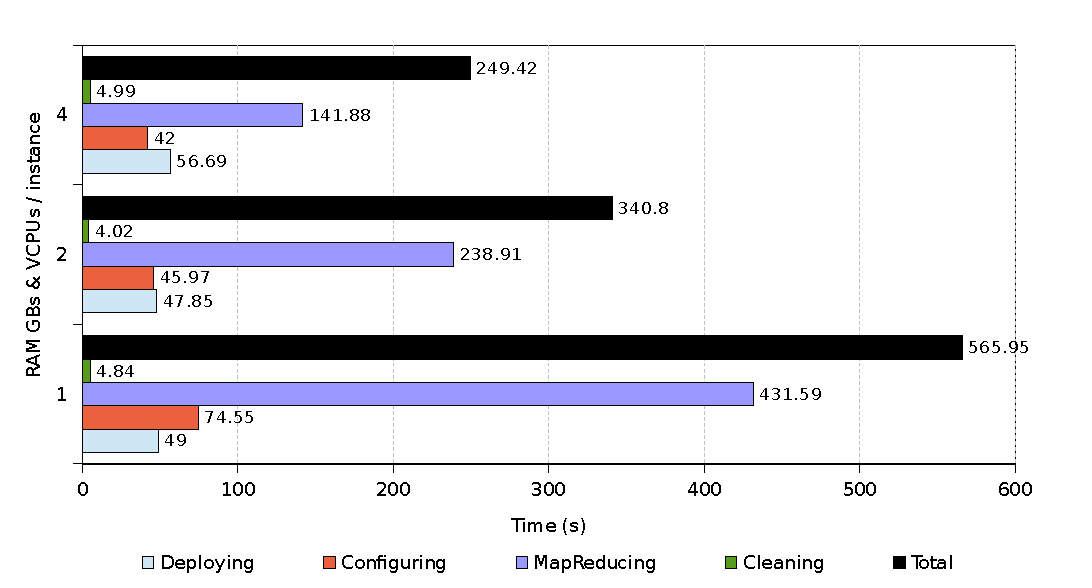
\includegraphics[width=0.98\textwidth]{imagenes/041.pdf}
\caption{Escalabilidad vertical}
\label{fig:escvertical}
\end{center}
\end{figure}

A la vista de esta figura, tal vez lo m\'as llamativo sean los tiempos de des\-plie\-gue y borrado, pudiendo considerarse pr\'acticamente constantes a pesar de aumentar la capacidad de c\'alculo de las instancias. Dicho de otro modo, la dificultad que supone desplegar o borrar un cl\'uster virtual en nuestro entorno depende exclusivamente del n\'umero de instancias o nodos virtuales ---conclusi\'on que ya hab\'iamos alcanzado previamente. Precisamente, hab\'iamos observado c\'omo la complejidad de configuraci\'on crec\'ia proporcionalmente con el tama\~no del cl\'uster. En este caso sucede lo contrario: al estar mejorando las caracter\'isticas t\'ecnicas de las dos instancias, los tiempos de configuraci\'on de Hadoop se ven l\'ogicamente reducidos. Es decir, la conclusi\'on revisada dicta que el tiempo de configuraci\'on var\'ia de forma directa con el n\'umero de instancias y de forma inversa con las capacidades operativas de las mismas. \newline

Los resultados contenidos en estas gr\'aficas demuestran que nuestra soluci\'on se comporta de modo m\'as eficaz cuando se mejora la capacidad de c\'omputo de las instancias ---escalabilidad vertical--- en vez de aumentar el tama\~no del cl\'uster virtual soporte ---escalabilidad horizontal. Este hecho se observa con claridad en las figuras \ref{fig:eschorizontal} y \ref{fig:escvertical} al comparar los casos extremos de prueba: ocho instancias de 1 GB de RAM frente a 4 GB de RAM y VCPUs por ins\-tan\-cia, respectivamente. Ambos casos distribuyen sendos clusters virtuales con las mismas caracter\'isticas de 8 VCPUs y 8 GB de RAM sobre nuestros nodos de prueba. Sin embargo, el tiempo de ejecuci\'on total es casi un \texttt{28\%} menor al mejorar las dos instancias (figura \ref{fig:escvertical}); esperable, en cierta medida, al ahorrar la sobrecarga de comunicaci\'on por la red. \newline

\begin{figure}[tbp]
\begin{center}
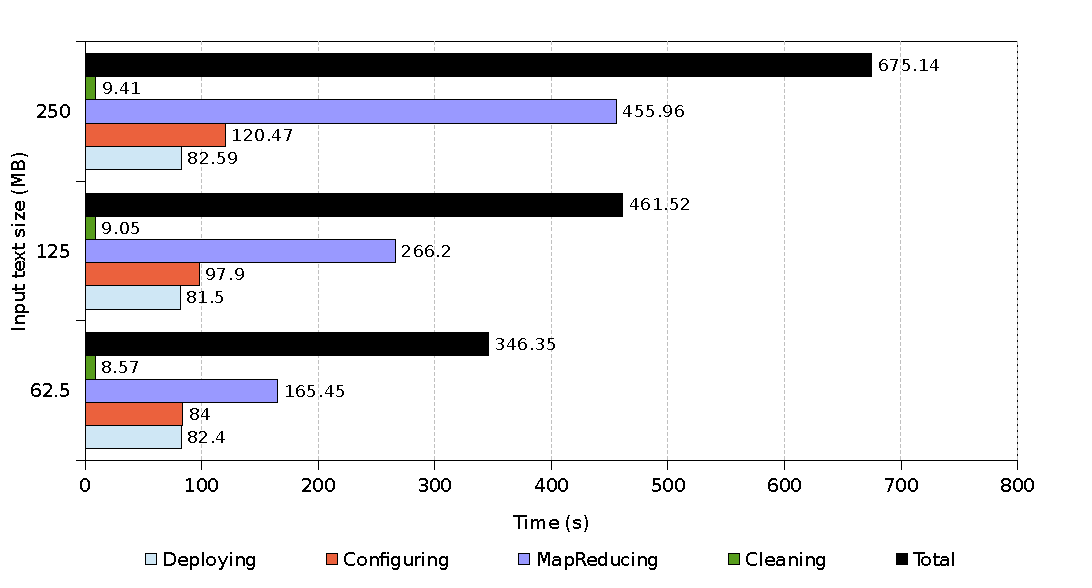
\includegraphics[width=0.98\textwidth]{imagenes/042.pdf}
\caption{Tama\~no de entrada frente a tiempo de ejecuci\'on}
\label{fig:evotemporal}
\end{center}
\end{figure}

La figura \ref{fig:evotemporal} muestra la evoluci\'on de los tiempos de ejecuci\'on al incrementar la magnitud de los datos a procesar. Como era de esperar, la duraci\'on de la etapa MapReduce y la duraci\'on total crecen en relaci\'on directa con el tama\~no de entrada, pero en menor medida. Los tiempos de despliegue y bo\-rra\-do se mantienen pr\'acticamente constantes en cada caso, mientras que el tiempo de configuraci\'on crece ligeramente, al englobar la descompresi\'on y posterior distribuci\'on de los ficheros de entrada sobre el cl\'uster Hadoop.
